\section{\secState{R}Motivation}\label{s:motivation}
\noindent The commercial potential of \emph{Unmanned Autonomous Systems} (UAS) is significant  enough to initiate one of the most significant changes in \emph{aviation} history \cite{airbusUTM2018blueprint}. The current \emph{usage} of UAS is limited by \emph{strict regulations} \cite{icao4444,icaoAnnex2,icaoAnnex11}. The goal is to enable \emph{full integration} of UAS in \emph{European airspace} by end of the year 2035 \cite{eurocontrol2018rpasatm}.


\begin{figure}[H]
    \centering
    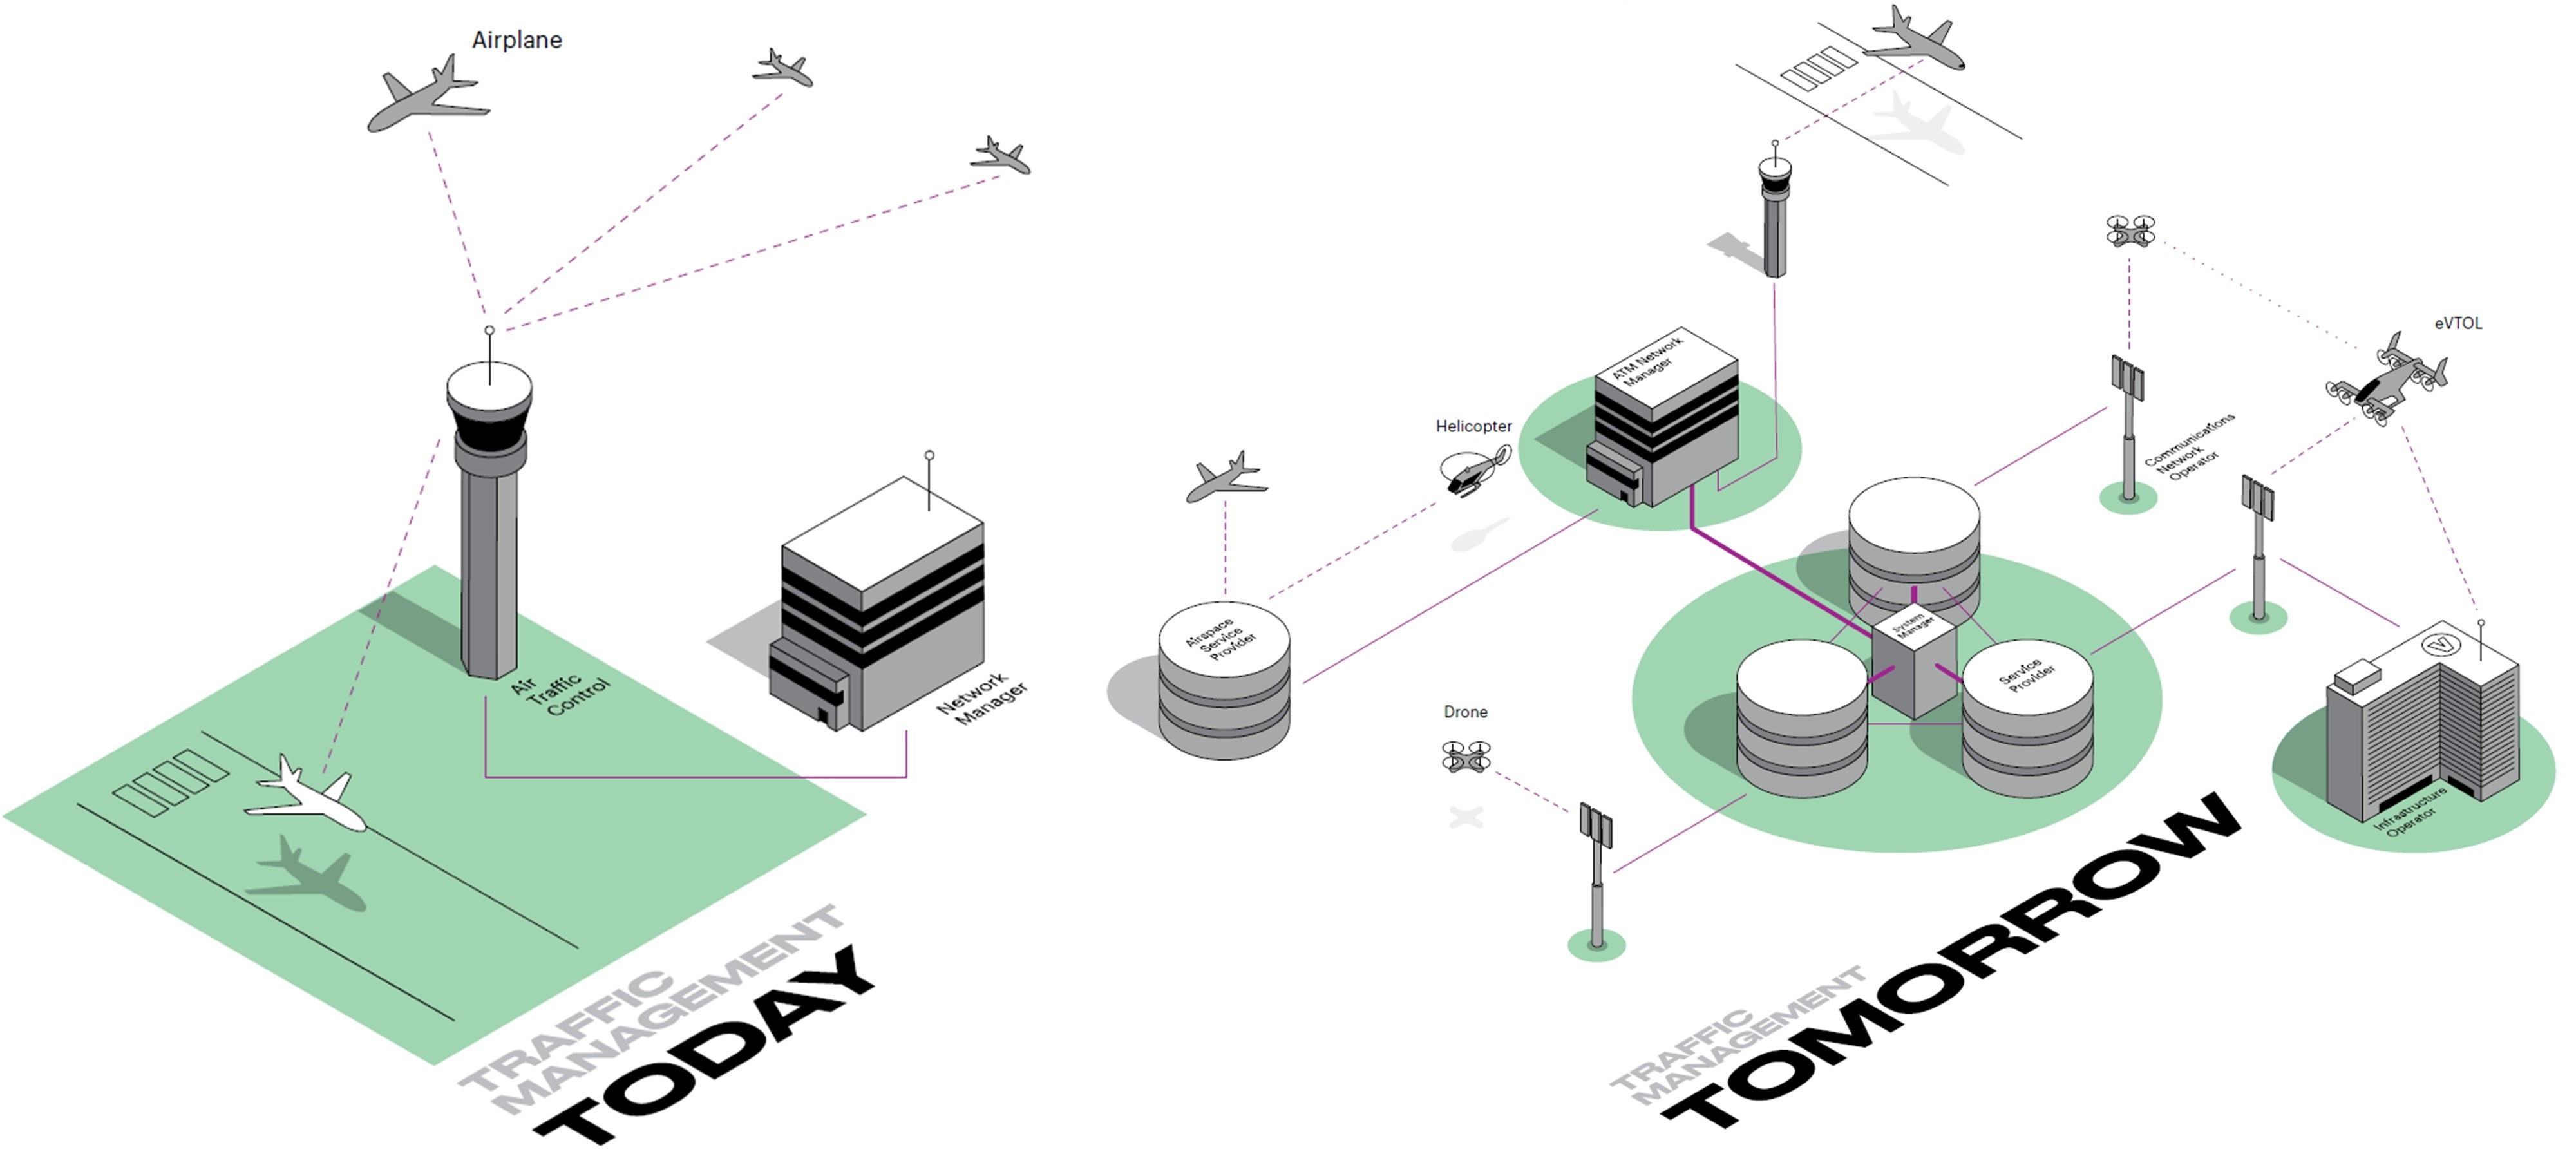
\includegraphics[width=0.9\textwidth]{\FIGDIR/I001TrafficManagement}
    \caption{Present and future \emph{Air Traffic Management} (ATC) \cite{airbusUTM2018blueprint}.}
    \label{fig:airTrafficManagementEvolution}
\end{figure}

\paragraph{UAS integraiton into Air Traffic:} The major effort is focused on \emph{Air Traffic Control} (ATC) changes. The \emph{actual} organization (sec. \ref{sec:AirspaceClassification}) and management (sec. \ref{sec:WellClear}) of airspace is centralized and \emph{human operated}.  

The \emph{ongoing changes} are shown in (fig. \ref{fig:airTrafficManagementEvolution}). The \emph{UAS Traffic Management} (UTM) (sec. \ref{sec:UTM}) complementing ATC is introduced to manage unmanned aviation. The additional traffic hubs, for UAS \emph{delivery \& transportation} services are added. The greatest change is on previously \emph{low-altitude uncontrolled} airspace, this space has new authority (UTM). The future UAS must implement mechanisms for \emph{event-based} navigation and avoidance (sec. \ref{sec:EventBasedAvoidance}).

Since 2014, there is a visible strong political support for developing rules on drones but regulations are harmonizing slowly. The European Aviation Safety Agency (EASA) has been tasked to develop a regulatory framework for drone operations and proposals for the regulation of "low-risk" UAV operations. In achieving this, EASA is working closely with the Joint Authorities for Regulation of Unmanned Systes (JARUS) \cite{jarus2016regulations}.

The \emph{operational rules} (sec. \ref{sec:AircraftOperationRules}) with \emph{rules of the air} \cite{icaoAnnex2} which are enforced now are simple. The \emph{future flight rules} (fig. \ref{fig:flightRulesIntro}) will be more complicated including the precise waypoint system and more complex missions. The future flight rules will be micro-managed by UTM. The example of such micro-management is shown in (sec. \ref{sec:UASTrafficManagement}, \ref{s:RuleEngineArchitecture}). 

The \emph{increase} of \emph{traffic density} increases the \emph{accident probability/severity}.  There are different threats endangering UAS, the \emph{obstacles} imposes eminent destruction threat, intruders can cooperate in mutual avoidance, the weather avoidance becomes more critical, the international/national authority can impose additional operational constraints. These threats needs to be well managed and prioritized to guarantee safe UAS operations.

\begin{figure}[H]
    \centering
    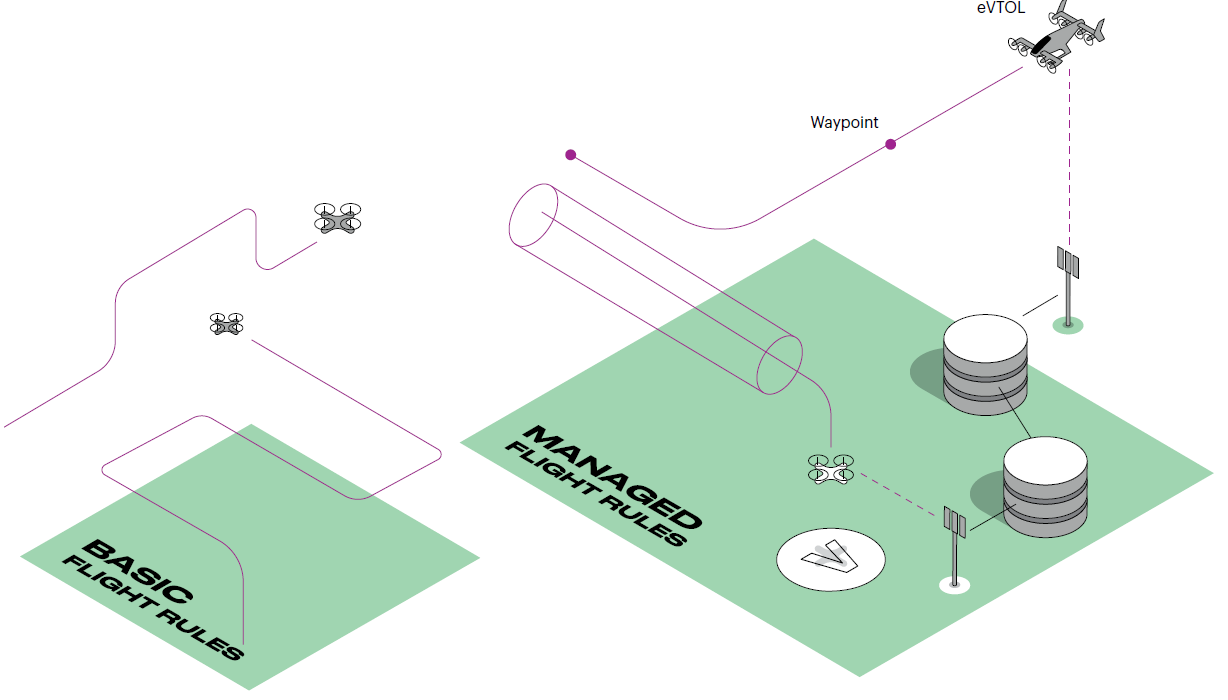
\includegraphics[width=0.8\textwidth]{\FIGDIR/I002FlightRules}
    \caption{Flight rules overview. \cite{airbusUTM2018blueprint}.}
    \label{fig:flightRulesIntro}
\end{figure}

\paragraph{Detect \& Avoid:} The other approach is bottom-up, that means the development of basic adaptable functionality to cover complex navigation/avoidance tasks in \emph{controlled airspace}. The intuitive definition of \emph{Detect \& Avoid} (DAA) functionality is given in (fig. \ref{fig:detectAdnAvoidIntroduction}).

\begin{figure}[H]
    \centering
    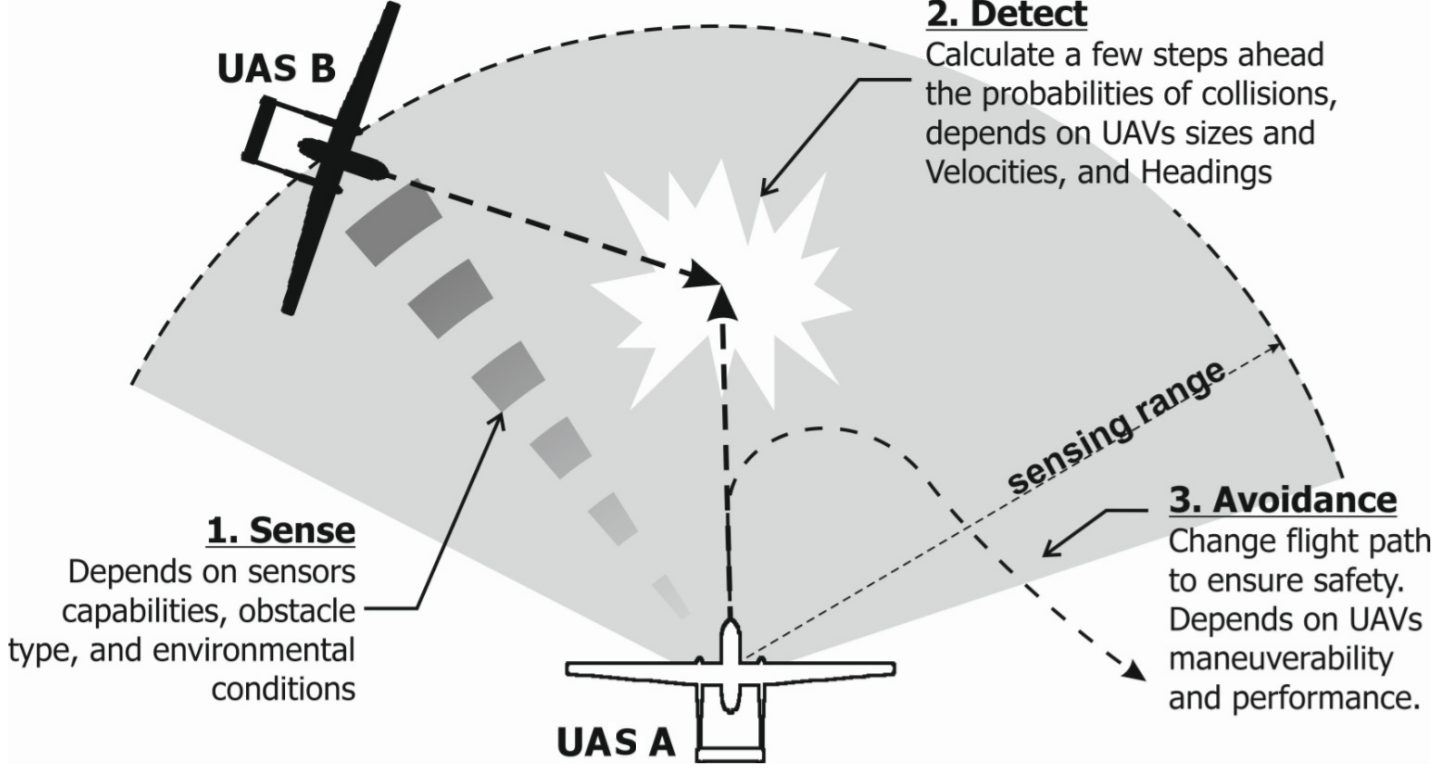
\includegraphics[width=0.6\textwidth]{\FIGDIR/I003DetectAndAvoid}
    \caption{\emph{Detect \& Avoid} (DAA) principle \cite{jenie2014velocity}.}
    \label{fig:detectAdnAvoidIntroduction}
\end{figure}

\noindent The DAA can be applied in short term (avoidance) and long term (navigation) tasks. It consist from three continuously repeating major steps:
\begin{enumerate}
    \item \emph{Sense} - the processing of intermediate sensor reading, the physical world approximation creation.
    
    \item \emph{Detect} - an addition of information from other sources to create complex situation assessment scenario, future possibilities projection and control strategy selection.
    
    \item \emph{Avoid} - execution of selected control strategy while checking possible changing events.
\end{enumerate}

The \emph{short term avoidance} (sec. \ref{s:aviudabceGridRun}) can be chained into \emph{long term navigation} (sec. \ref{s:missionControlRun}). This long term navigation can be used to solve \emph{UTM/ATM} imposed constraints, under assumption that there is sufficient \emph{data fusion} (sec. \ref{s:sensorFusion}).

\paragraph{Challenge Motivation:} Both \emph{Air Traffic Control} and \emph{Detect \& Avoid} requires a tool to assess possible UAS maneuvering:

\begin{enumerate}
    \item \emph{Air Traffic Control} needs to know the UAS maneuvering capabilities in order to \emph{validate} feasibility of \emph{issued orders} and to predict future \emph{trajectory} for \emph{collision prevention}.
    
    \item \emph{Detect \& Avoid} needs to calculate feasible \emph{system constraints feasible maneuvering strategy} in finite time to ensure own safety. 
\end{enumerate}

\paragraph{Reach Sets:} These challenges are addressable by employment of \emph{reach sets} (sec. \ref{s:ReachSets}). The \emph{reach set} is self-validating set of possible maneuvering strategies for some initial UAS state and some time-period. 

To guarantee finite time evaluation, the discretization of \emph{operation space} (sec. \ref{s:AvoidanceGrid}) and \emph{movement discretization} (sec. \ref{sec:MovementAutomatonBackground}) needs to be introduced. The discretization gives finite countable sets of choices, therefore it also guarantees finite time evaluation process.

Our \emph{implementation} of \emph{reach set approximation} (sec. \ref{s:reachSet}) enables to encode some sought behavioral patterns as natural properties (sec. \ref{s:constrainedTrajectoryExpansion}). This enables to generate specific task oriented \emph{reach set approximation} for navigation (sec. \ref{s:chaoticReachSet}), avoidance (sec. \ref{s:harmonicReachSet}), UTM behavior predictions (sec. \ref{sec:collisionCase}). 

